% show 我们用的概念的定义
\begin{frame}{Terminologies}% {Optional Subtitle}

\begin{figure}
    \centering
    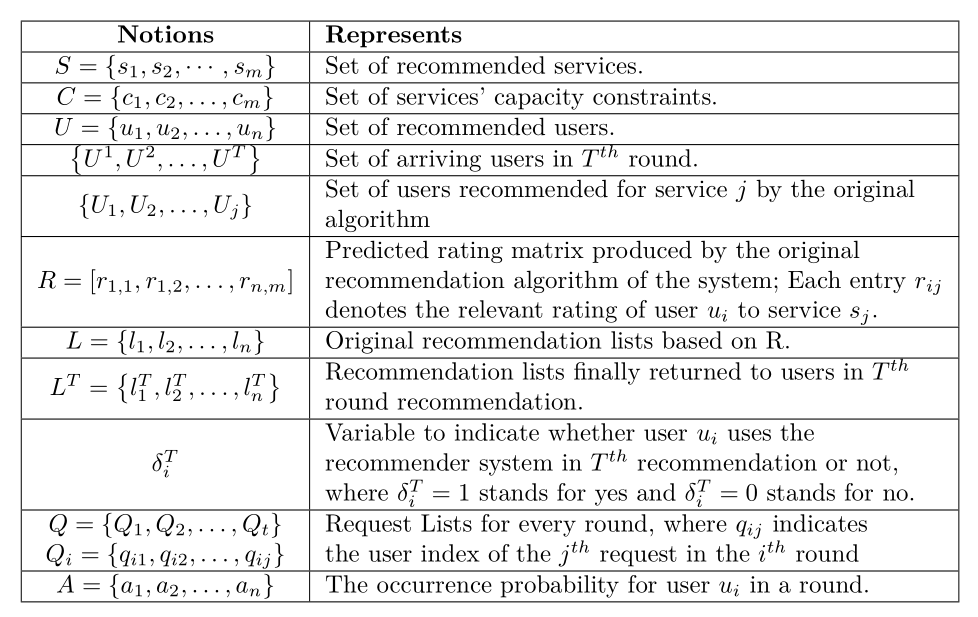
\includegraphics[width=0.9\textwidth]{img/notion.png}
    \caption{Basic Notions}
    \label{notion}
\end{figure}
   
\end{frame}

%%%%%%%%%

\begin{frame}{Definition}% {Optional Subtitle}
\begin{block}{Definition 1: Ideal Probability}
\begin{equation}
p_{j}^{T}=\frac{\sum_{u_{i} \in U_{j}} \sum_{t=0}^{T} \delta_{i}^{t} \cdot  \operatorname{Is\_In}\left(s_{j}, l_{i}^{t}, N\right)}{\sum_{u_{i} \in U_{j}} \sum_{t=0}^{T} \delta_{i}^{t}}
\end{equation}
\end{block}
% question: sum to average or average to sum when counting probability
\begin{block}{Definition 2: Actual Probability} 
\begin{equation}
p_{i, j}^{T}=\frac{\sum_{t=0}^{T} \delta_{i}^{t} \cdot \operatorname{Is\_In}\left(s_{j}, l_{i}^{t}, N\right)}{\sum_{t=0}^{T} \delta_{i}^{t}}
\end{equation}
where $\delta_{i}^{t}$ indicates the possibility that user $i$ is the owner of a request in the $t^{\text{th}}$ round.
\end{block}
where
\begin{equation}\operatorname{Is\_In}\left(s_{j}, l i s t, N\right)=\left\{\begin{array}{l}0 \text { if } s_{j} \text { is not in the top } N \text { sub-list of list } \\ 1 \text { if } s_{j} \text { is in the top } N \text { sub-list of list }\end{array}\right.\end{equation}
\end{frame}

\begin{frame}{Definition}% {Optional Subtitle}

\begin{block}{Definition 3: Service Fairness Degree}
  Fairness degree of user $u_{i}$ on service $s_{j}$ up to $T^{t h}$ round recommendation:
\begin{equation}
F_{i, j}^{T}=\frac{p_{i, j}^{T}-p_{j}^{T}}{p_{j}^{T}}
\label{eqn:def_fairness}
\end{equation}

\end{block}
This definition gives a metric for fairness. The larger $|F|$ is,
the less fairness the recommendation has.

And we can define the Service Fairness Degree among the Top-N list of one user.

\begin{block}{Definition 4: Top-N Overall Fairness Degree}
  Overall fairness degree of user $u_{i}$ up to $T^{t h}$ round recommendation:
\begin{equation}
F_{i}^{T}=\sum_{s_{j} \in l(N)_{i}} F_{i, j}^{T}
\end{equation}

\end{block}
\end{frame}


\begin{frame}{Recommendation Quality Metric}% {Optional Subtitle}

\begin{block}{Definition 5:  Recommendation Quality Metric}
 Quality of outputted recommendation list $l_{i}^{T}$ of user $u_{i}$ on $T^{\text {th }}$ round recommendation:
\begin{equation}
    q_{i}^{T}=\frac{\sum_{s_{j} \in l(N)_{i} \cap l(N)_{i}^{t}} \frac{r_{i, j}}{\log _{2}\left(p_{i, j}^{T}+1\right)}}{r_{i, l(N)_{i}[0]}}
\end{equation}
where $l(N)_{i}[0]$ represents the subscript index of the service appearing at the top position of $l(N)_{i},$ and $p_{i, j}^{T}$ is the position of service $s_{j}$ in $l(N)_{i}$
\end{block}

\begin{enumerate}
    \item Considering the quality of $l(N)_{i}$, namely the top-N list;
    \item Normalizing the quality score with the highest rating of $l(N)_{i}$ as the denominator.
\end{enumerate}

 

\end{frame}
